\begin{frame}{Das MVC-Konzept}{Grundlegendes (Vgl. \cite{judt2017} S. 3)}
    \begin{itemize}
        \item Bildet Klassenkombination zur Konstruktion von Benutzerschnittstellen ab
        \begin{itemize}
            \item Modell (Model) -- Anwendungsobjekt
            \item Sicht (View) -- Darstellung des Modells auf dem Bildschirm (ggf. mehrfach)
            \item Steuerung (Controller) -- Definiert Reaktion der Benutzerschnittstelle auf Eingaben
        \end{itemize}
        \item MVC gehört zu den Entwurfsmustern, das selbst mehrere starke Entwurfsmuster vereinigt, unter anderem Beobachter, Kompositum und Strategie
    \end{itemize}
\end{frame}

\begin{frame}{MVC}{Muster 1 -- Beobachter (\textit{Observer})}
    \begin{figure}
    \centering
    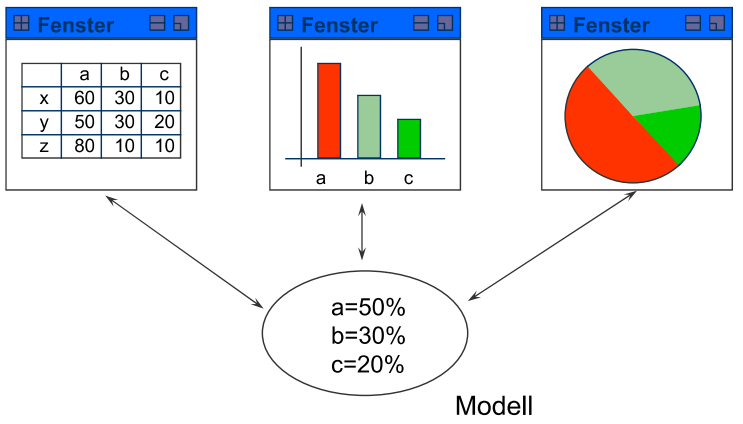
\includegraphics[height=5cm]{graph/mvc_observer}
    \caption*{Quelle: \cite{judt2017}, S. 4}
    \end{figure}
\end{frame}

\begin{frame}{MVC}{Observer Muster (Vgl. \cite{judt2017} S. 5)}
    \begin{itemize}
        \item Beziehung zwischen Sichten und Modell entspricht dem "`Beobachter"' Muster
        \begin{itemize}
            \item Zwischen Modell ("`Subjekt"') und der Sicht ("`Beobachter"') gibt es Registrierungs- und Benachrichtigungs-Interaktionen
            \item Bei Änderungen im Modell werden die Sichten benachrichtigt. Jede Sicht aktualisiert sich unabhängig voneinander durch Zugriff auf das Modell
            \item Das Modell weiß nicht, wie die Sichten die Daten verwenden. Die Sichten wissen nicht voneinander (Entkopplung)
        \end{itemize}
    \end{itemize}
\end{frame}

\begin{frame}{MVC}{Muster 2 -- Kompositum (Siehe \cite{judt2017} S. 6)}  
    \begin{itemize}
        \item Sichten können als zusammengesetzte Sicht geschachtelt sein
        \item Wie schon besprochen, basiert das Swing Framework auf dem Entwurfsmuster des Kompositums durch Verwendung von \textit{Containern} und \textit{Komponenten}
        \item Somit erfüllt jede Swing GUI Anwendung dieses Entwurfsmuster
    \end{itemize}
\end{frame}

\begin{frame}{MVC}{Muster 3 -- Strategie (Siehe \cite{judt2017} S. 7)}
    \begin{itemize}
        \item Zwischen Steuerung und Sicht entsteht eine Beziehung, die das Strategie-Entwurfsmuster verwendet
        \begin{itemize}
            \item Von der Steuerung existieren mehrere Unterklassen, die unterschiedliche Antwortstrategien abbilden. Zum Beispiel können Tastatureingaben anders behandelt werden oder andere Kommandos benutzt werden
            \item Jede Sicht kann individuell auswählen, welche Antwortstrategie sie nutzt. Diese kann auch dynamisch ausgewählt werden
        \end{itemize}
    \end{itemize}
\end{frame}

\begin{frame}{Beispiel}{Für eine MVC Anwendung}
    \begin{itemize}
        \item Es sollen Daten für einen Student erfasst werden
        \item Ein Student besteht aus:
        \begin{itemize}
            \item Einer ID
            \item Dem Vornamen
            \item Dem Nachnamen
        \end{itemize}
    \end{itemize}
\end{frame}

\begin{frame}{Beispiel}{Für eine MVC Anwendung}
    \begin{itemize}
        \item Jetzt soll eine Fensteranwendung entworfen werden in der:
        \begin{itemize}
            \item Die Daten für einen Studenten gespeichert werden
            \item Die einzelnen Attribute angezeigt werden (In Labels)
            \item Für jedes Attribut zusätzlich ein Textfeld existiert in denen ein neuer Wert eingegeben werden kann
            \item Durch Klick auf einen Button, sollen die Daten des Studenten aktualisiert werden (mit den neuen Werten aus den Textfeldern)
        \end{itemize}
        \item \textbf{Welcher Teil der Anwendung ist Model/View/Controller?}
    \end{itemize}
\end{frame}